\section{ER-Diagramm}\label{er-diagramm}
In diesem Kapitel wird die Datenbankstruktur des Projekts dargestellt.\\
\begin{figure}[h]
    \centering
    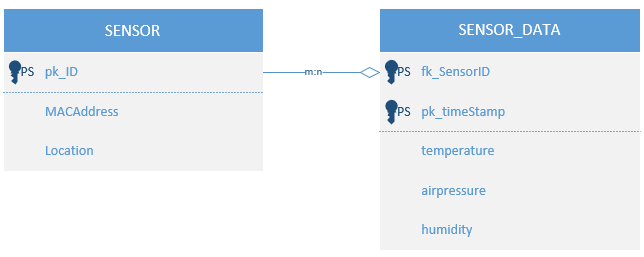
\includegraphics[width=1\linewidth]{img/erd}
    \caption[ER-Diagramm des Projekts]{ER-Diagramm des Projekts (eigene Darstellung)}
    \label{fig:erd}
\end{figure}

In \autoref{fig:erd} ist das ER-Diagramm des Projekts dargestellt. Die Datenbankstruktur ist bewusst simpel aber erweiterbar gehalten.
\subsection*{SENSOR}
Die Tabelle Sensor beinhaltet alle Informationen über die Sensoren des Systems.
Neben einer vom System vergebenen ID sind Informationen über die MAC-Adresse und den Standort enthalten.
Die MAC-Adresse wird bei jeder Request vom System zur Identifikation mitgeschickt und dient im Backend der Zuordnung von Messwerten zu Sensoren. Die MAC-Adresse wird als String gespeichert, es findet jedoch im Backend eine Überprüfung statt, die sicherstellt dass keine fehlerhafte Formatierung möglich ist.
Die Spalte \enquote{Location} ermöglicht die Zuordnung eines Standorts zu einer Messstation. Dieser Wert kann im Frontend nur durch den Administrator festgelegt werden, weshalb hier keine besondere Datenvalidierung notwendig ist und die Speicherung als String die größtmögliche Flexibilität bietet.
\subsection*{SENSOR\_DATA}
%TODO add kommentar bzgl. C->unix-timestamp=sekunden, JS->unix=millisekunden
%TODO make vereinigung -> unique kriterium again
%TODO request hinzugefügt -> datenbank
In dieser Tabelle werden die einzelnen Datensätze gespeichert. Ein Datensatz besteht standardmäßig aus einem Zeitstempel, und je einem Messwert für Temperatur, Luftdruck und -Feuchtigkeit. Die Einzigartigkeit eines Datensatzes wird durch die Vereinigung der Sensor-ID und des Zeitstempels sichergestellt. Der Sensor überträgt die oben genannten Daten zusätzlich zu seiner eigenen MAC-Adresse. Im Backend wird vor dem Speichern des Messwerts anhand der MAC-Adresse die Sensor-ID ermittelt (wenn der Sensor bereits bekannt ist) oder neu vergeben und dem Request hinzugefügt, mit dem die Daten dann in die Datenbank eingefügt werden. Zeitstempel und die drei Messwerte sind hierbei numerisch gewählt, wobei integer als Datentyp ausreichend ist, um die möglichen Zeitstempel abzudecken und beispielsweise float genügt, um die möglichen Messwerte mit Komma zu speichern. Im Backend erfolgt eine Validierung der Daten, die verhindert dass verfälschte Messwerte oder Zeitstempel (zum Beispiel in Folge eines Messfehlers) in die Datenbank geraten.\\